\documentclass[11  pt]{article} 
\usepackage[lmargin=1in,rmargin=1.75in,bmargin=1in,tmargin=1in]{geometry}  


% For hyperlinking everything
\usepackage{hyperref}
\hypersetup{
	colorlinks=true, %set true if you want colored links
	linktoc=all,     %set to all if you want both sections and subsections linked
	linkcolor=blue,  %choose some color if you want links to stand out
}


\usepackage[latin1]{inputenc}
\usepackage{amsmath}
\usepackage{mathrsfs}  
\usepackage{amsfonts}
\usepackage{amssymb}
\usepackage{graphicx}
\usepackage{subfig}
\usepackage{caption}
\usepackage{algorithm}
%\usepackage{algcompatible}
%\usepackage{algorithmicx}
\usepackage{algpseudocode}

\usepackage{titlesec}
\titleformat{\section}{\fontfamily{lmss}\fontsize{14}{15}\bfseries}{\thesection}{1em}{}
\titleformat{\subsection}{\fontfamily{lmss}\fontsize{12}{15}\bfseries}{\thesubsection}{1em}{}




\usepackage{amsthm}

\newtheoremstyle{noit}
{10pt}% <Space above>
{10pt}% <Space below>
{}% <Body font>
{}% <Indent amount>
{\bfseries}% <Theorem head font>
{.}% <Punctuation after theorem head>
{.5em}% <Space after theorem headi>
{}% <Theorem head spec (can be left empty, meaning `normal')>

\newtheoremstyle{example}
{10pt}% <Space above>
{10pt}% <Space below>
{}% <Body font>
{20pt}% <Indent amount>
{\bfseries}% <Theorem head font>
{.}% <Punctuation after theorem head>
{.5em}% <Space after theorem headi>
{}% <Theorem head spec (can be left empty, meaning `normal')>


\newtheoremstyle{indented}{20pt}{20pt}{\addtolength{\leftskip}{2.5em}}{}{\bfseries}{.}{.5em}{}


\newtheorem{theorem}{Theorem}
\numberwithin{theorem}{section}
\newtheorem{lemma}[theorem]{Lemma}
\newtheorem{corollary}[theorem]{Corollary}
\newtheorem{observation}{Observation}
%\numberwithin{observation}{section}
%\numberwithin{definition}{section}
\newtheorem{conjecture}{Conjecture}
\newtheorem{Qu}{Question}
\newcommand{\QU}{\begin{Qu}\normalfont}

\theoremstyle{noit}
\newtheorem{fact}{Fact}
\newtheorem{definition}{Definition}

\theoremstyle{indented}
\newtheorem{example}{Example}

\theoremstyle{indented}
\newtheorem{problem}{Problem}


%\newenvironment{proof}{\noindent{\bf Proof:} \hspace*{1em}}{
%    \hspace*{\fill} $\Box$ }
%\newenvironment{proof_of}[1]{\noindent {\bf Proof of #1:}
%    \hspace*{1em} }{\hspace*{\fill} $\Box$ }
%\newenvironment{proof_claim}{\begin{quotation} \noindent}{
%    \hspace*{\fill} $\diamond$ \end{quotation}}
\newcommand{\vs}[1]{\vspace{#1}}

\newcommand{\lecture}[2]{
 \noindent
\begin{center}
	\framebox{
		\vbox{
			\hbox to 5.78in { {\bf CSCE 411: Design and Analysis of Algorithms} \hfill  }
			\vspace{2mm}
			\hbox to 5.78in { {\Large \hfill Lecture #1\hfill} }
			\vspace{2mm}
			\hbox to 5.78in { {\it Date: #2 \hfill Lecturer: Nate Veldt} }
		}
	}
\end{center}
\vspace*{4mm}
}


\newcommand{\hw}[2]{
	\noindent
	\begin{center}
		\framebox{
			\vbox{
				\hbox to 5.78in { {\bf CSCE 411: Design and Analysis of Algorithms} \hfill  }
				\vspace{2mm}
				\hbox to 5.78in { {\Large \hfill Homework #1\hfill} }
				\vspace{2mm}
				\hbox to 5.78in { {\it Due date: #2 \hfil} }
			}
		}
	\end{center}
	\vspace*{4mm}
}



\newcommand{\under}[1]{\underline{\hspace{#1}}}
\setlength{\parindent}{0em}

%\usepackage[tagged]{accessibility}

% Graph terms
\newcommand{\vol}{\textbf{vol}}
\newcommand{\cut}{\textbf{cut}}


% Matrices
\newcommand{\mA}{\textbf{A}}
\newcommand{\mB}{\textbf{B}}

% vectors
\newcommand{\ve}{\textbf{e}}
\newcommand{\vx}{\textbf{x}}


% Other
\newcommand{\calN}{\mathcal{N}}

\usepackage{mathtools}
\DeclarePairedDelimiter\ceil{\lceil}{\rceil}
\DeclarePairedDelimiter\floor{\lfloor}{\rfloor}


\newcommand*{\aitem}{ \item[{
\includegraphics[width=0.8cm,height=0.5cm]{../../Lectures/figures/A}} ]  }
\newcommand*{\bitem}{ \item[{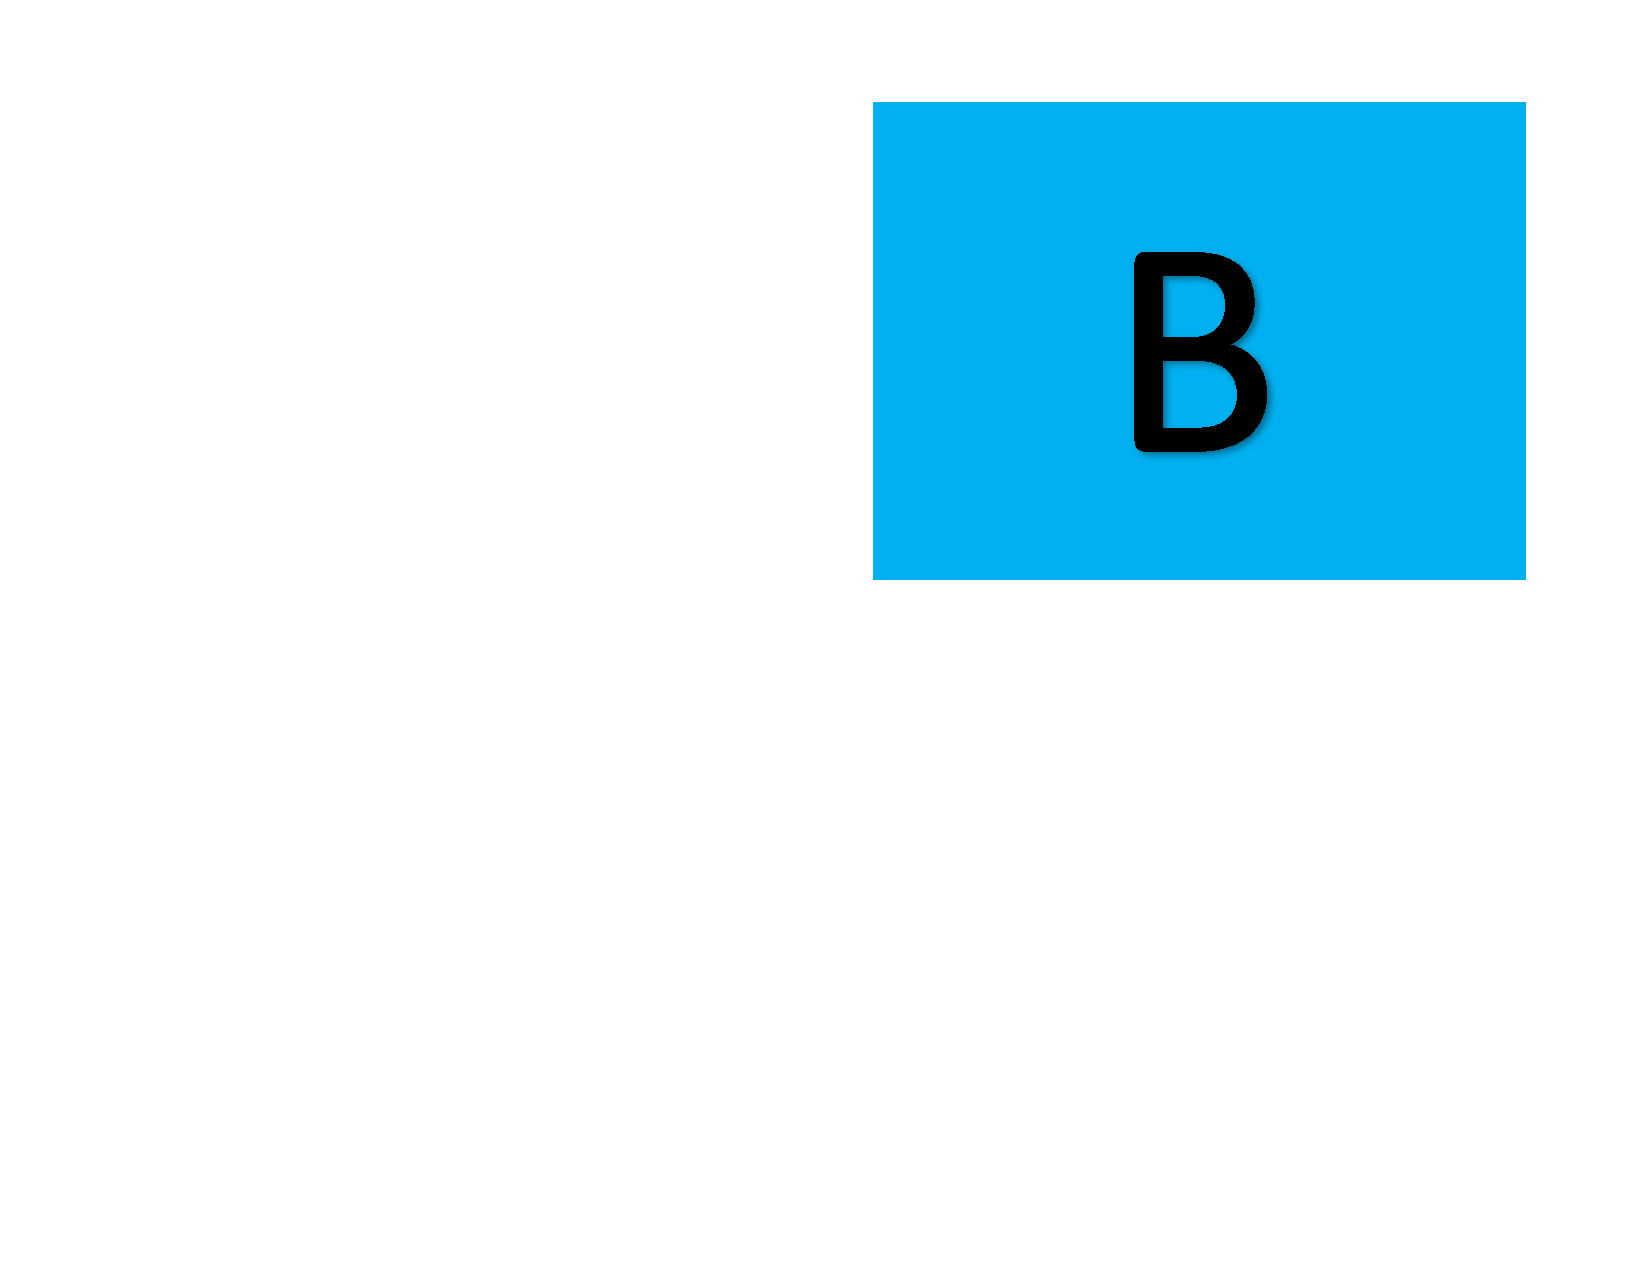
\includegraphics[width=0.8cm,height=0.5cm]{../../Lectures/figures/B}} ]  }
\newcommand*{\citem}{ \item[{
\includegraphics[width=0.8cm,height=0.5cm]{../../Lectures/figures/C}} ]  }
\newcommand*{\ditem}{ \item[{
\includegraphics[width=0.8cm,height=0.5cm]{../../Lectures/figures/D}} ]  }
\newcommand*{\eitem}{ \item[{
\includegraphics[width=0.8cm,height=0.5cm]{../../Lectures/figures/E}} ]  }
\newcommand*{\fitem}{ \item[{
\includegraphics[width=0.8cm,height=0.5cm]{../../Lectures/figures/F}} ]  }


\newcommand{\hide}[1]{\underline{\phantom{#1 #1}}}

\usepackage{setspace}

\onehalfspacing

\begin{document}
	
	\lecture{: Approximation Algorithms and Optimization}{Week 14}
	\textbf{Course Logistics}
	\begin{itemize}
		\item CLRS Chapter 34
		\item Last homework due Friday
	\end{itemize}
	
	
		\section{Linear programming}
		
		A linear program is a mathematical optimization problem with 
	\begin{itemize}
		\item A linear objective function
		\item Linear constraints
	\end{itemize}

We will use $x_i$ to denote variables---unknowns that we need to find to make the objective function as large as possible, and such that the constraints hold. \\

\paragraph{Examples} 

\newpage

		
		\paragraph{Warm-up problem (from CLRS).} 
As a politician seeking approval ratings, you would like the
support of 50 urban voters, 100 suburban voters, 25 rural
voters. 
		
For each $\$1$ spent advertising one of the following policies,
the resulting effects are:
		
\begin{center}
\begin{tabular}{|c|c|c|c|}
\hline
\textbf{Policy} & \textbf{Urban} & \textbf{Suburban} & \textbf{Rural} \\
\hline
Zombie apocalypse & -2 & +5 & -3 \\
Shark with lasers & +8 & +2 & -5 \\
Flying cars roads & 0 & 0 & +10 \\
Dolphins voting & +10 & 0 & -2 \\
\hline
\end{tabular}
\end{center}		

Minimize the amount spent to achieve the desired voter support. 
How can we write this as an algorithmic or mathematic problem?		


\vs{1cm}
Create variables:
\begin{itemize}
\item
Let \hide{$x_1$} be the money spent on ads for preparing for a zombie apocalypse
\item
Let \hide{$x_2$} be the money spent on ads for sharks with lasers
\item
Let \hide{$x_3$} be the money spent on ads for roads for flying cars
\item
Let \hide{$x_4$} be the money spent on ads for allowing dolphins to vote
\end{itemize}
Then the objective of the problem is:

\vs{2cm}
The constraints of the problem are: 

\vs{4cm}
		
	
\newpage

\paragraph{Another example problem.} 
The students of \textbf{CSCE 411} are managing their semester project portfolios, which involve three types of projects:

\begin{itemize}
    \item \textbf{Project A:} Basic Algorithms.
    \item \textbf{Project B:} Graph Algorithms.
    \item \textbf{Project C:} Complexity. 
\end{itemize}

Each project type earns a different amount of grade contribution points and consumes a mix of three limited resources: \textit{Self-Study Time}, \textit{Computation Credits}, and \textit{Team Collaboration Hours}.

\begin{center}
\begin{tabular}{|c|c|c|c|c|}
\hline
\textbf{Project Type} & \textbf{Grade Points} & \textbf{Time (hours)} & \textbf{Credits (units)} & \textbf{Collab Hours} \\
\hline
A & 10 & 5 & 3 & 2 \\
B & 12 & 6 & 2 & 4 \\
C & 8 & 4 & 4 & 3 \\
\hline
\end{tabular}
\end{center}

The semester budget for a student is:
\begin{itemize}
    \item Maximum 60 hours of Self-Study Time.
    \item Maximum 30 Computation Credits.
    \item Maximum 36 Collaboration Hours.
\end{itemize}

Additionally, the professor requires that at least 2 projects from each type be completed for a balanced learning experience.
Given the budget and these constraints, devise a project plan to maximize the grade. 

\vs{1cm}
Write a linear program for this problem.

\vfill
\newpage

%\section*{Linear Program (Primal Form)}
%
%Let:
%\begin{itemize}
    %\item \( x_1 \) = number of Project A completed.
    %\item \( x_2 \) = number of Project B completed.
    %\item \( x_3 \) = number of Project C completed.
%\end{itemize}
%
%The linear program is:
%
%\[
%\begin{aligned}
%\text{Maximize:} \quad & 10x_1 + 12x_2 + 8x_3 \\
%\text{Subject to:} \quad & 5x_1 + 6x_2 + 4x_3 \leq 60 \quad (\text{Time limit}) \\
%& 3x_1 + 2x_2 + 4x_3 \leq 30 \quad (\text{Computation credits limit}) \\
%& 2x_1 + 4x_2 + 3x_3 \leq 36 \quad (\text{Collaboration hours limit}) \\
%& x_1 \geq 2, \quad x_2 \geq 2, \quad x_3 \geq 2 \quad (\text{Minimum project count}) \\
%& x_1, x_2, x_3 \geq 0 \quad (\text{Non-negativity})
%\end{aligned}
%\]

\section{Types of Linear Programs}
Linear programs have many variations:
\begin{itemize}
	\item The objective function can be a maximization or a minimization problem
	\item The constraints can be equality or inequalities
	\item Often times, the variables will be greater than or equal to zero
\end{itemize}

Actually, we can perform different conversions to

\begin{itemize}
	\item Turn a maximization problem into a minimization problem \\
	
	\vs{2cm}
	
	\item Turn an equality constraint into inequality constraints \\
	
		\vs{2cm}
	
	
	\item Turn an inequality constraint into an equality constraint \\
	
		\vs{2cm}
	
	\item Turn an unconstrained variable into positive variables \\
\end{itemize}


\vfill

\textbf{Important Fact:} A linear program can be solved in polynomial time.

\newpage

\section{Graph problems as mathematical optimization problem}
We can write the maximum $s$-$t$ flow problem as the following optimization problem:


\vfill

The weighted vertex cover problem can be written as the following optimization problem:
\vfill

\begin{Qu}
	Which of the above two problems is a linear program?
	\begin{itemize}
		\aitem The first
		\bitem The second
		\citem Both
		\ditem Neither
	\end{itemize}
\end{Qu}

\newpage



\section{Linear Programming Relaxation for Weighted Vertex Cover}
This is the integer program for the weighted vertex cover problem:



\vfill

\begin{Qu}
	Let $\hat{C}$ be the optimal solution value to the linear programming relaxation of the weighted vertex cover integer program, and let $\mathcal{C}^*$ be the optimal solution to the weighted vertex cover problem. Which of the following is always true?
	\begin{itemize}
		\aitem $\hat{C} \leq C^*$
		\bitem $\hat{C} \geq C^*$
		\citem $\hat{C} < C^*$
		\ditem $\hat{C} > C^*$
		\eitem $\hat{C} = C^*$
	\end{itemize}
\end{Qu}

\newpage
\section{The Algorithm}
	$\textsc{WeightedVertexCoverApprox}(G = (V,E))$
\begin{enumerate}
	\item Solve the linear programming relaxation of the weighted vertex cover problem
	\item For each node $v \in V$, if $x_v \geq 1/2$, add $v$ to a node set $S$. In other words, define
	\begin{equation*}
		S = \{v \in V \colon x_v \geq 1/2\}
	\end{equation*}
	\item Return $S$ as a vertex cover
\end{enumerate}
\begin{theorem}
	Let $C^*$ be the weight of the minimum weighted vertex cover of $G$. The algorithm \textsc{WeightedVertexCoverApprox} runs in polynomial time in terms of the size of $G$ and outputs a vertex cover $S \subseteq V$ satisfying $\sum_{v \in S} w_v\leq 2C^*$. 
\end{theorem}
	
	
	
	
	
	
	
	
	
	\section{Approximation Algorithms for Optimization Problems}
	There are so many hard problems out there without known polynomial time solutions! Is all hope lost? What do we do?\\
	
	Approximation algorithms ``quickly'' find an answer that is ``close'' to the solution. \\ \\
	
	\vs{3cm} 
	
	We are now focused on optimization problems, rather than just their \emph{decision} versions.
	\paragraph{Definition}
	Let $Q$ be a computational minimization problem (e.g., find a minimum vertex cover, find a minimum $s$-$t$ cut) and assume that $C^*$ is the optimal (minimum) solution to the problem. An \hide{approx algorithm} for $Q$ with approximation factor $p$ is an algorithm that 
	\begin{itemize}
		\item Runs in %polynomial time
		\item Outputs a solution value $C$ that is guaranteed to satisfy % $\frac{C}{C^*} \leq p$.\\
	\end{itemize}
	
	\vfill
	
	\begin{Qu}
		What is a lower bound we must assume holds for the value of $p$ when defining an approximation algorithm?
		\begin{itemize}
			\aitem No lower bound is needed, $p$ can be any real number
			\bitem $ p \geq -1$
			\citem $p \geq 0$
			\ditem $p \geq 1$
			\eitem $p \geq C^*$
		\end{itemize}
	\end{Qu}
	\vs{1cm}
	
	We can also have approximation algorithms for maximization problems, but in this case $C^*$ represents the \emph{maximum} value (i.e., the solution) for the problem and \hide{$p \leq 1$.} %We will focus on the minimization case here.\\ \\
	
	
	
	\newpage
	
	\paragraph{Wait, is this even possible?}
	We want to guarantee that $\frac{C}{C^*}$ is small in polynomial time, but finding $C^*$ is NP-hard. How can we do that? \\
	
	To design an approximation algorithm, we need two pieces:
	\begin{enumerate}
		\item \hide{Lower bound.} A procedure for finding a value $\hat{C}$ that satisfies \hide{$\hat{C} \leq C^*$}
		\begin{itemize}
			\item It should take polynomial time \\
			\item This method \hide{does not} solve the original problem, but is often related
		\end{itemize}
		\item \hide{Upper bound.} An algorithm for the original problem that returns \\
		
		a suboptimal solution \hide{$C \geq C^*$} \\ \\
		\begin{itemize}
			\item It should take polynomial time \\
			\item This method often: \\
		\end{itemize}
	\end{enumerate}
	
	We then must prove that \hide{$\frac{C}{\hat{C}} \leq p$} and this provides a $p$-approximation! 
	
	\vfill
	
	
	\textbf{Caveat.} Often, the lower bounding procedure is \emph{explicit}: there is an actual algorithm that computes the lower bound, and then the upper bounding algorithm explicitly uses the lower bound. However, in some cases no explicit lower bound is computed, and instead one shows implicitly that the upper bounding algorithm has to provide a solution that is better than some lower bound, even though the lower bound isn't computed explicitly. This can be tricky, but it is often possible!
	
	\newpage
	\section{Matchings and Vertex Covers}
	Let $G = (V,E)$ be an undirected and unweighted graph. \\
	
	A matching $\mathcal{M} \subseteq E$ is a set of edges such that no two edges share the same node. \\ 
	
	A vertex cover $\mathcal{C} \subseteq V$ is a set of nodes such that each edge $(u,v) \in E$ has at least one node in $\mathcal{C} \subseteq V$.\\
	\vspace{5cm} 
	
	
	\begin{lemma}
		Let $\mathcal{M}$ be a matching of $G$ and $\mathcal{C}$ be a vertex cover. Then $|\mathcal{M}| \leq |\mathcal{C}|$.
	\end{lemma}

	
	%Assume that is not the case, and that $\mathcal{M}$ has more edges than $\mathcal{C}$ has nodes.  \\
	%	
	%	Let $S$ be the set of nodes adjacent to an edge in $\mathcal{M}$. Since all of these nodes touch exactly one edge in $\mathcal{M}$, we know that $|\mathcal{M}| = \frac{|S|}{2}$.
	

	
	\newpage
	\section{The approximation algorithm for vertex cover}
	A matching $\mathcal{M} \subseteq E$ is a \emph{maximal} matching if for every edge $e \in E - \mathcal{M}$, $\mathcal{M} \cup \{e\}$ is no longer a matching. \\
	
	
	\vspace{8cm}
	
	
	\textbf{The algorithm}\\
	
	$\textsc{VertexCoverApprox}(G = (V,E))$
	\begin{enumerate}
		\item Compute a maximal matching $\mathcal{M}$ of $G$:
		\begin{itemize}
			\item Set $F = E$, $\mathcal{M} = \emptyset$
			\item While $|F| > 0$
			\begin{itemize}
				\item Add any edge $e \in F$ to $\mathcal{M}$
				\item For each remaining $f \in F$, if $|e \cap f| > 0$, remove $f$ from $F$
			\end{itemize}
		\end{itemize}
		\item Let $S$ be the set of nodes adjacent to an edge in $\mathcal{M}$
		\item Return $S$\\
	\end{enumerate}
	
	\newpage
	\begin{theorem}
		Let $C^*$ be the minimum sized vertex cover of $G$. The algorithm \textsc{VertexCoverApprox} runs in polynomial time in terms of the size of $G$ and outputs a vertex cover $S \subseteq V$ satisfying $|S| \leq 2C^*$. Thus, this is a 2-approximation algorithm for vertex cover.
	\end{theorem}


	

\end{document}